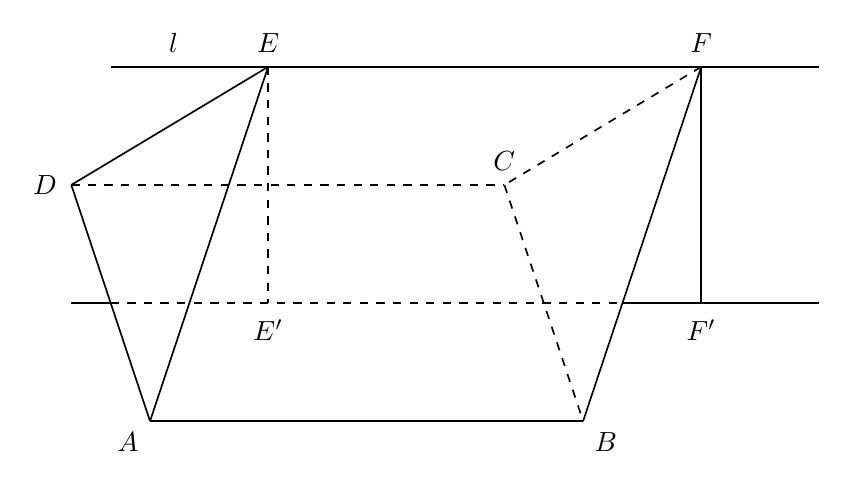
\begin{tikzpicture}[x=1cm,y=1cm,font=\normalsize,
  edge/.style={draw=black,line width=.6pt},
  hid/.style={draw=black,line width=.6pt,dashed},
  lbl/.style={font=\normalsize,inner sep=2pt}]
% projection positions (schematic, perspective view of square ABCD)
\coordinate (lL) at (0.5,4.5);
\coordinate (lR) at (9.5,4.5);
\coordinate (E) at (2.5,4.5);
\coordinate (F) at (8.0,4.5);
\coordinate (Ep) at (2.5,1.5);
\coordinate (Fp) at (8.0,1.5);
\coordinate (D) at (0.0,3.0);
\coordinate (C) at (5.5,3.0);
\coordinate (A) at (1.0,0.0);
\coordinate (B) at (6.5,0.0);
\coordinate (lowL) at (0.0,1.5);
\coordinate (lowM1) at (0.5,1.5);
\coordinate (lowM2) at (7.0,1.5);
\coordinate (lowR) at (9.5,1.5);
% top line l
\draw[edge] (lL) -- (lR);
% lower reference line through E',F' (solid ends, dashed middle)
\draw[edge] (lowL) -- (lowM1);
\draw[hid] (lowM1) -- (lowM2);
\draw[edge] (lowM2) -- (lowR);
% verticals
\draw[hid] (E) -- (Ep);
\draw[edge] (F) -- (Fp);
% square top edge (hidden) and bottom edge
\draw[hid] (D) -- (C);
\draw[edge] (A) -- (B);
% left side and diagonals
\draw[edge] (D) -- (A);
\draw[edge] (E) -- (D);
\draw[edge] (E) -- (A);
\draw[edge] (F) -- (B);
\draw[hid] (F) -- (C);
\draw[hid] (C) -- (B);
% labels (offset to avoid touching strokes)
\node[lbl,above=3pt] at (1.3,4.5) {$l$};
\node[lbl,above=3pt] at (E) {$E$};
\node[lbl,above=3pt] at (F) {$F$};
\node[lbl,below=4pt] at (Ep) {$E'$};
\node[lbl,below=4pt] at (Fp) {$F'$};
\node[lbl,left=3pt] at (D) {$D$};
\node[lbl,above=3pt] at (C) {$C$};
\node[lbl,below left=2pt] at (A) {$A$};
\node[lbl,below right=2pt] at (B) {$B$};
\end{tikzpicture}
